\chapter{Coreference resolution}
\label{chapter:Coreference resolution}
\section{History}

First algorithms for coreference and anaphora resolution date in the '70 of the last century. The first algorithm was published by Hobbs[46,47] in 1976.This algorithm, a pronominal anaphora resolution algorithm, resolved pronouns "he", "she",  "it". Basically, this algorithm was based on syntax rules and heuristics and these rules are:

\begin{itemize}
	\item anaphora and antecedent should corresponds in their gender and number
	\item antecedent of a pronoun is the first NP that can be reached with fewer number of steps
	\item the algorithm uses common sense knowledge (candidate selection)
\end{itemize}

Hobbs tested his algorithm manually in three different gender texts (historical, novels and news). He claimed that the naive approach algorithm, without using common sense knowledge, achieves accuracy 88\%, and with common sense knowledge  and with "careful" selection of antecedents achieves accuracy more than 91\%. These accuracies, the algorithm achieved because Hobbs assumed that the parser that build the syntax structure of sentences is a perfect parser.   

In practice, a pronominal anaphora resolution algorithm is hard to achieve accuracy of around 90\%, because does not exist a perfect parser and does not exist a tool that has a common sense knowledge.

\newpage
\begin{algorithm}[H]
\caption{Hobbs's algorithm}\label{alg:Hobbs}
\begin{algorithmic}[1]
\State Begin at the $NP$ node immediately dominating the pronoun.
\State Go up the tree to the first $NP$ or $S$ node encountered. Call this node $X$, and call the path used to reach it $p$.
\State Traverse all branches below node $X$ to the left of path $p$ in a left-to-right, breadth first fashion. Propose as the antecedent any $NP$ node that is encountered which has an $NP$ or $S$ node between it and $X$.
\If { node $X$ is the highest node in the sentence} 
	\State traverse the surface parse trees of previous sentences in the text in order of recency, the most recent first; each tree is traversed in a left-to-right, breadth-first manner, and when an $NP$ is encountered, it is proposed as antecedent
\Else
	\State (X is not the highest node in the sentence) continue to step 9.
\EndIf
\State From node X, go up the tree to the first NP or S node encountered. Call this new node X, and call the path traversed to reach it p.
\If {X is an NP node and if the path p to X did not pass through the N node that X immediately dominates}
     \State propose X as the antecedent
\EndIf
\State Traverse all branches below node X to the left of path p in a left-to-right, breadth first manner. Propose any NP node encountered as the antecedent
\If {X is an S node}
    \State traverse all branches of node X to the right of path p in a left-to-right, breadth first manner, but do not go below any NP or S node encountered.
    \State Propose any NP node encountered as the antecedent.
\EndIf
\State Go to step 4
\end{algorithmic}
\end{algorithm}

\begin{figure}[h]
	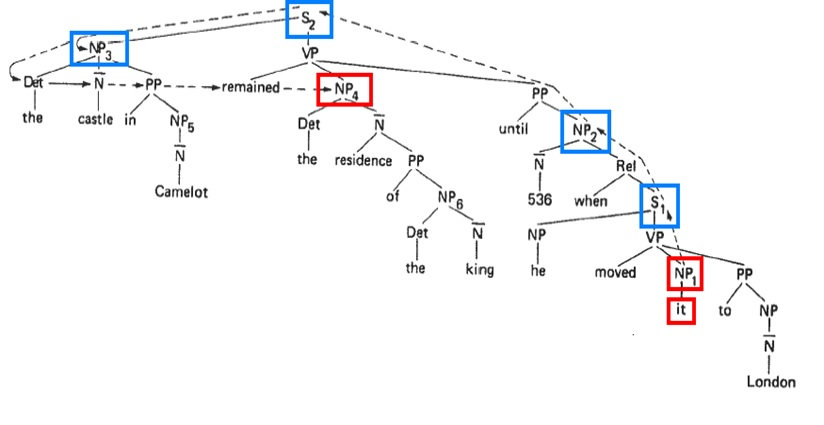
\includegraphics[scale=0.60]{hobbs.jpg} 
 	\caption{Simulation of Hobbs's Algorithm [30,31] }
	\label{Figure 5}
\end{figure}

The trend of building coreference and anaphora resolution algorithms based on common sense knowledge and rules continued in the years 90s(1990-1995). Another characteristic of this period is that did not exist an metric to measure performance of anaphora and coreference resolution systems. Because of this, scientist defined specific evaluation metrics for their algorithms in anaphora and coreference resolution.

In this period scientists Barbara J. Grosz,Aravind K. Joshi, Scott Weinstein [48] publish a theory in coreference resolution. This theory, the centring theory, go further in analysis of coreference and anaphora. To resolve anaphora in their theoretical model they add "relationships among focus of attention, choice of referring expression and perceived coherence of utterances within a discourse segment" [14]. This is the first theoretical model that uses the content of the text in anaphora and coreference resolution.

In mid 90s scientists started to apply coreference and anaphora resolution in information extraction. 

When scientists started to develop coreference resolution systems they needed a standard of coreference resolution algorithms. To have a standard measurement metrics for evaluation of coreference and anaphora resolution algorithms, the computational linguistic community built and annotated a corpus, and defined evaluation measurements, which are the official standards of coreference and anaphora resolution. The corpus and standards were published in the MUC-6 (Message Understanding Conference) conference. The corpus consisted of 60 English language newswire articles. Two years latter the community published a new corpus MUC-7, which was an update of the previous corpus. These two corpuses are most used and famous corpuses. After publishing these two corpuses, different NLP communities published corpuses and evaluation metrics of coreference resolution. Another known corpus, which is used in the computational linguistic is the Automatic Content Extraction (ACE1) corpus. During this period the community was concentrated in building a base theory of coreference resolution. As a result, they defined standards in annotation schemas and the terminology (e.g. markable detection, mention) that is required in coreference and anaphora resolution. 

In the beginning of the year 2000, scientists started using machine learning algorithms in coreference and anaphora resolution. In these methods, they used morphological and structural features: number, gender and part of speech  classes of noun phrases to achieve higher accuracy in the resolution. The researcher Soon et al. (2001) to resolve anaphora generated a set of 12 features. In this set of features Ng and Cardie added 53 other features, including positional, morphological, lexical, syntactic, semantic and even pragmatic features. These methods achieved accuracy around 60-67\%. 

 Meanwhile, the computational linguistic community started to get more interested in coreference and anaphora resolution. As a result, new corpuses in different domains and languages were published. Now, there are annotated and published corpuses in domains: scientific articles, dialogues, news and clinical domain; and in languages:Arabic, Chinese, Dutch, English, French,Italian, Japanese,Spanish and Tibetan language. 

The community realised that a coreference resolution algorithm perform well in one corpus, but achieves poor results in another corpus. This property of algorithms leads to new perception of coreference resolution. Scientists started to develop corpus based coreference and anaphora resolution algorithms. In the last ten years, scientists are using domain specific features and syntactic rules. Depending on the corpus, the results of the best methods achieve accuracy around 70\% in anaphora resolution. [43,65]

\section{Coreference resolution in biomedical domain}

Coreference resolution is believed that helps relationship extraction. This inspired, in 2008, the BioNLP community to build a corpus, with research paper's abstracts, to support other information extraction in biomedical domain. Until now a public corpus with full text articles with protein coreference annotation does not exist.

\section{The state of the art in protein coreference resolution} 

In 2011 was organized a competition in Protein Coreference Resolution. The purpose of the task was to evaluate the effect of coreference resolution in biomedical relationship extraction. In the competition the results in protein coreference resolution were not good enough, the best performing algorithm in protein coreference resolution had an accuracy of 34.1\%. These results were too low to improve relationship extraction tasks in biomedical domain.[1] Organizers of the competition also provided detailed results of best performing algorithms, which are shown in Table 3.1.
\newpage
\begin{table}[h]
  \begin{center}
     \begin{tabular}{|l C{2cm} C{2cm} C{2cm}|} 
	 	\hline
  		& Precision & Recall & F-score \\ [1ex] 
 		\hline
 		1st place & 73.26 & 22.18 & 34.05 \\ [1ex]
 		\hline
 		2nd place & 54.45 & 21.48 & 30.96 \\[1ex]
  		\hline
 		3rd place & 63.22 & 19.37 & 29.65 \\ [1ex]
  		\hline
	\end{tabular}
  \end{center} 
  \caption{ Results of BioNLP Protein coreference resolution competition [1]}
  \label{table2}
\end{table}

After the competition some research groups were interested to improve the results of protein coreference resolution. One year later, in 2012, were published two papers in protein coreference resolution. In one of the papers authors use semantic classification and rules to resolve protein coreference and achieved an accuracy of 51.3\%. In the second paper authors use an hybrid approach of rules and SVMs and it achieves an accuracy of 60.9\%. This algorithm is the current state of the art in protein coreference resolution.
 
 In the table 3.2, I present results of the best performing algorithms in protein coreference resolution.
\begin{table}[h]
  \begin{center}
 	\begin{tabular}{|l C{2cm} C{2cm} C{2cm}|} 
 		\hline
  		& Precision & Recall & F-score \\ [1ex] 
 		\hline
 		Hybrid approach & 55.6 & 67.2 & 60.9 \\ [1ex] 
 		\hline
 		Event miner & 50.4 & 62.7 & 55.9 \\ [1ex] 
 		\hline
 		Semantic classification & 52.2 & 50.2 & 51.3 \\ [1ex] 
 		\hline
 		Reconcile & 73.3 & 22.2 & 34.1 \\ [1ex] 
 		\hline
	\end{tabular}
  \end{center} 
  \caption{Results of the best performing algorithms in Protein coreference resolution}
  \label{table3.2}
\end{table}

A full text article corpus with protein coreference annotation does not exist. To evaluate the results of my algorithm in the protein coreference resolution in full text articles I have annotated 8 full text articles, and results of my algorithm in this corpus will be the first  results in the protein coreference resolution in full text.
 
\section{Available tools for biomedical information extraction}

To complete the coreference task, I needed supporting NLP tools for preprocessing and structuring the data set.

For coreference resolution, I used tools that are trained in biomedical domain, because they have better performance than other tools. In the following paragraphs I will describe the tools that i used in my system.

I used the deep parser "ENJU parser", which is trained in biomedical data [50]. Empirically, it is shown that this parser achieves better results in biomedical domain than other parsers [63]. This parser is a Head-driven phrase structure grammar (HPSG)parser. HSPG parsers use semantic and syntactic rules, as well as dictionary to build the tree structure of the sentence[51-57]. The average time of parsing a sentence is 500ms. This parser achieves precision 87.85\% and recall 86.85\% on the Penn Treebank and the average parsing time is 360 ms per sentence [66].

\begin{figure}[h]
  \begin{center}
	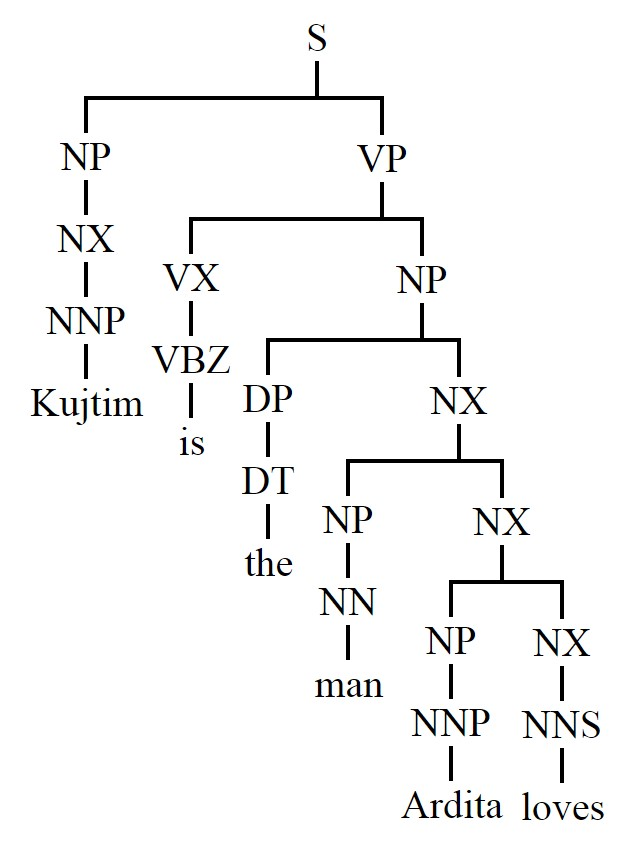
\includegraphics[scale=0.25]{Enju_output.jpg} 
 	\caption{Simulation of Hobbs's Algorithm [30] }
	\label{Figure 6}
  \end{center}
\end{figure}

An advantage of HPSG parsers is that they give rich linguistic informations. The Enju parser returns the syntactic structure of the sentence in tree. This structure is returned as XML object. In each internal node (not leaf) of the XML object are included these informations: syntactic category (verb, noun phrase preposition,...), extra syntax category (coordinate clause, subordinate clause), and a unique identifier for the node. 

For each token, leaf node of the tree, the parser provides information about the following linguistic characteristics: unique identifier of the token, syntactic category, Penn Treebank-style part of speech tag, base form, and for each of part of speech gives its characteristics (words, punctuations). For example for verb, gives following information: the person, the number, the tense, aspect and voice(passive/active). 

\newpage
\begin{figure}[h]
   \begin{center}
		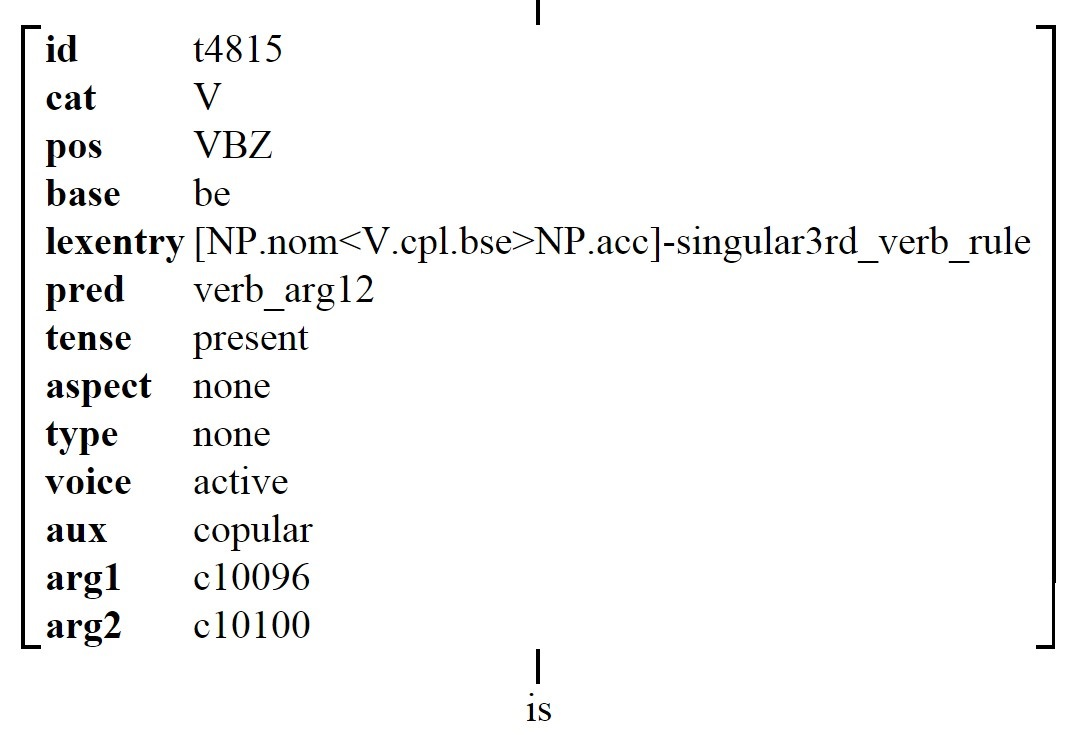
\includegraphics[scale=0.25]{Extended.jpg} 
 		\caption[Information that \emph{Enju parser} gives for the token \emph{is}]{Information that \emph{Enju parser} gives for the token \emph{is}}
		\label{Figure 7}
	\end{center}
\end{figure}
 
Another tool that I used in this thesis is the sentence splitter, GENIA sentence splitter (GeniaSS) [59]. This sentence splitter receives a text (a text file) as input and returns array of sentences (a file where each sentence is written in a specific line). This sentence splitter is trained on supervised learning method using maximum entropy modelling; and it is implemented in C++ [61]. 

GeniaSS is high accurate parser sentence splitter in the Biomedical domain, it achieves an F-score of 99.7 on 200 unseen GENIA corpus.[15]
